%% bare_jrnl.tex
%% V1.4b
%% 2015/08/26
%% by Michael Shell
%% see http://www.michaelshell.org/
%% for current contact information.
%%
%% This is a skeleton file demonstrating the use of IEEEtran.cls
%% (requires IEEEtran.cls version 1.8b or later) with an IEEE
%% journal paper.
%%
%% Support sites:
%% http://www.michaelshell.org/tex/ieeetran/
%% http://www.ctan.org/pkg/ieeetran
%% and
%% http://www.ieee.org/

%%*************************************************************************
%% Legal Notice:
%% This code is offered as-is without any warranty either expressed or
%% implied; without even the implied warranty of MERCHANTABILITY or
%% FITNESS FOR A PARTICULAR PURPOSE! 
%% User assumes all risk.
%% In no event shall the IEEE or any contributor to this code be liable for
%% any damages or losses, including, but not limited to, incidental,
%% consequential, or any other damages, resulting from the use or misuse
%% of any information contained here.
%%
%% All comments are the opinions of their respective authors and are not
%% necessarily endorsed by the IEEE.
%%
%% This work is distributed under the LaTeX Project Public License (LPPL)
%% ( http://www.latex-project.org/ ) version 1.3, and may be freely used,
%% distributed and modified. A copy of the LPPL, version 1.3, is included
%% in the base LaTeX documentation of all distributions of LaTeX released
%% 2003/12/01 or later.
%% Retain all contribution notices and credits.
%% ** Modified files should be clearly indicated as such, including  **
%% ** renaming them and changing author support contact information. **
%%*************************************************************************


% *** Authors should verify (and, if needed, correct) their LaTeX system  ***
% *** with the testflow diagnostic prior to trusting their LaTeX platform ***
% *** with production work. The IEEE's font choices and paper sizes can   ***
% *** trigger bugs that do not appear when using other class files.       ***                          ***
% The testflow support page is at:
% http://www.michaelshell.org/tex/testflow/

% If IEEEtran.cls has not been installed into the LaTeX system files,
% manually specify the path to it like:
\documentclass[journal]{IEEEtran}





% Some very useful LaTeX packages include:
% (uncomment the ones you want to load)


% *** MISC UTILITY PACKAGES ***
%
%\usepackage{ifpdf}
% Heiko Oberdiek's ifpdf.sty is very useful if you need conditional
% compilation based on whether the output is pdf or dvi.
% usage:
% \ifpdf
%   % pdf code
% \else
%   % dvi code
% \fi
% The latest version of ifpdf.sty can be obtained from:
% http://www.ctan.org/pkg/ifpdf
% Also, note that IEEEtran.cls V1.7 and later provides a builtin
% \ifCLASSINFOpdf conditional that works the same way.
% When switching from latex to pdflatex and vice-versa, the compiler may
% have to be run twice to clear warning/error messages.






% *** CITATION PACKAGES ***
%
\usepackage{cite}
% cite.sty was written by Donald Arseneau
% V1.6 and later of IEEEtran pre-defines the format of the cite.sty package
% \cite{} output to follow that of the IEEE. Loading the cite package will
% result in citation numbers being automatically sorted and properly
% "compressed/ranged". e.g., [1], [9], [2], [7], [5], [6] without using
% cite.sty will become [1], [2], [5]--[7], [9] using cite.sty. cite.sty's
% \cite will automatically add leading space, if needed. Use cite.sty's
% noadjust option (cite.sty V3.8 and later) if you want to turn this off
% such as if a citation ever needs to be enclosed in parenthesis.
% cite.sty is already installed on most LaTeX systems. Be sure and use
% version 5.0 (2009-03-20) and later if using hyperref.sty.
% The latest version can be obtained at:
% http://www.ctan.org/pkg/cite
% The documentation is contained in the cite.sty file itself.






% *** GRAPHICS RELATED PACKAGES ***
%

\ifCLASSINFOpdf
  \usepackage[pdftex]{graphicx}
  \graphicspath{ {./images/} }
  \DeclareGraphicsExtensions{.pdf,.jpeg,.png}
\else

  \usepackage[dvips]{graphicx}
  \graphicspath{{../eps/}}
  \DeclareGraphicsExtensions{.eps}
\fi
% graphicx was written by David Carlisle and Sebastian Rahtz. It is
% required if you want graphics, photos, etc. graphicx.sty is already
% installed on most LaTeX systems. The latest version and documentation
% can be obtained at: 
% http://www.ctan.org/pkg/graphicx
% Another good source of documentation is "Using Imported Graphics in
% LaTeX2e" by Keith Reckdahl which can be found at:
% http://www.ctan.org/pkg/epslatex
%
% latex, and pdflatex in dvi mode, support graphics in encapsulated
% postscript (.eps) format. pdflatex in pdf mode supports graphics
% in .pdf, .jpeg, .png and .mps (metapost) formats. Users should ensure
% that all non-photo figures use a vector format (.eps, .pdf, .mps) and
% not a bitmapped formats (.jpeg, .png). The IEEE frowns on bitmapped formats
% which can result in "jaggedy"/blurry rendering of lines and letters as
% well as large increases in file sizes.
%
% You can find documentation about the pdfTeX application at:
% http://www.tug.org/applications/pdftex




\usepackage{lscape}
\usepackage{rotating}
\usepackage{tikz}
% *** MATH PACKAGES ***
%
\usepackage{amsmath}
% A popular package from the American Mathematical Society that provides
% many useful and powerful commands for dealing with mathematics.
%
% Note that the amsmath package sets \interdisplaylinepenalty to 10000
% thus preventing page breaks from occurring within multiline equations. Use:
%\interdisplaylinepenalty=2500
% after loading amsmath to restore such page breaks as IEEEtran.cls normally
% does. amsmath.sty is already installed on most LaTeX systems. The latest
% version and documentation can be obtained at:
% http://www.ctan.org/pkg/amsmath





% *** SPECIALIZED LIST PACKAGES ***
%
\usepackage{algorithmic}
% algorithmic.sty was written by Peter Williams and Rogerio Brito.
% This package provides an algorithmic environment fo describing algorithms.
% You can use the algorithmic environment in-text or within a figure
% environment to provide for a floating algorithm. Do NOT use the algorithm
% floating environment provided by algorithm.sty (by the same authors) or
% algorithm2e.sty (by Christophe Fiorio) as the IEEE does not use dedicated
% algorithm float types and packages that provide these will not provide
% correct IEEE style captions. The latest version and documentation of
% algorithmic.sty can be obtained at:
% http://www.ctan.org/pkg/algorithms
% Also of interest may be the (relatively newer and more customizable)
% algorithmicx.sty package by Szasz Janos:
% http://www.ctan.org/pkg/algorithmicx




% *** ALIGNMENT PACKAGES ***
%
\usepackage{array}
% Frank Mittelbach's and David Carlisle's array.sty patches and improves
% the standard LaTeX2e array and tabular environments to provide better
% appearance and additional user controls. As the default LaTeX2e table
% generation code is lacking to the point of almost being broken with
% respect to the quality of the end results, all users are strongly
% advised to use an enhanced (at the very least that provided by array.sty)
% set of table tools. array.sty is already installed on most systems. The
% latest version and documentation can be obtained at:
% http://www.ctan.org/pkg/array


% IEEEtran contains the IEEEeqnarray family of commands that can be used to
% generate multiline equations as well as matrices, tables, etc., of high
% quality.




% *** SUBFIGURE PACKAGES ***
\ifCLASSOPTIONcompsoc
  \usepackage[caption=false,font=normalsize,labelfont=sf,textfont=sf]{subfig}
\else
  \usepackage[caption=false,font=footnotesize]{subfig}
\fi
% subfig.sty, written by Steven Douglas Cochran, is the modern replacement
% for subfigure.sty, the latter of which is no longer maintained and is
% incompatible with some LaTeX packages including fixltx2e. However,
% subfig.sty requires and automatically loads Axel Sommerfeldt's caption.sty
% which will override IEEEtran.cls' handling of captions and this will result
% in non-IEEE style figure/table captions. To prevent this problem, be sure
% and invoke subfig.sty's "caption=false" package option (available since
% subfig.sty version 1.3, 2005/06/28) as this is will preserve IEEEtran.cls
% handling of captions.
% Note that the Computer Society format requires a larger sans serif font
% than the serif footnote size font used in traditional IEEE formatting
% and thus the need to invoke different subfig.sty package options depending
% on whether compsoc mode has been enabled.
%
% The latest version and documentation of subfig.sty can be obtained at:
% http://www.ctan.org/pkg/subfig




% *** FLOAT PACKAGES ***
%
\usepackage{fixltx2e}
% fixltx2e, the successor to the earlier fix2col.sty, was written by
% Frank Mittelbach and David Carlisle. This package corrects a few problems
% in the LaTeX2e kernel, the most notable of which is that in current
% LaTeX2e releases, the ordering of single and double column floats is not
% guaranteed to be preserved. Thus, an unpatched LaTeX2e can allow a
% single column figure to be placed prior to an earlier double column
% figure.
% Be aware that LaTeX2e kernels dated 2015 and later have fixltx2e.sty's
% corrections already built into the system in which case a warning will
% be issued if an attempt is made to load fixltx2e.sty as it is no longer
% needed.
% The latest version and documentation can be found at:
% http://www.ctan.org/pkg/fixltx2e


%\usepackage{stfloats}
% stfloats.sty was written by Sigitas Tolusis. This package gives LaTeX2e
% the ability to do double column floats at the bottom of the page as well
% as the top. (e.g., "\begin{figure*}[!b]" is not normally possible in
% LaTeX2e). It also provides a command:
%\fnbelowfloat
% to enable the placement of footnotes below bottom floats (the standard
% LaTeX2e kernel puts them above bottom floats). This is an invasive package
% which rewrites many portions of the LaTeX2e float routines. It may not work
% with other packages that modify the LaTeX2e float routines. The latest
% version and documentation can be obtained at:
% http://www.ctan.org/pkg/stfloats
% Do not use the stfloats baselinefloat ability as the IEEE does not allow
% \baselineskip to stretch. Authors submitting work to the IEEE should note
% that the IEEE rarely uses double column equations and that authors should try
% to avoid such use. Do not be tempted to use the cuted.sty or midfloat.sty
% packages (also by Sigitas Tolusis) as the IEEE does not format its papers in
% such ways.
% Do not attempt to use stfloats with fixltx2e as they are incompatible.
% Instead, use Morten Hogholm'a dblfloatfix which combines the features
% of both fixltx2e and stfloats:
%
% \usepackage{dblfloatfix}
% The latest version can be found at:
% http://www.ctan.org/pkg/dblfloatfix




%\ifCLASSOPTIONcaptionsoff
%  \usepackage[nomarkers]{endfloat}
% \let\MYoriglatexcaption\caption
% \renewcommand{\caption}[2][\relax]{\MYoriglatexcaption[#2]{#2}}
%\fi
% endfloat.sty was written by James Darrell McCauley, Jeff Goldberg and 
% Axel Sommerfeldt. This package may be useful when used in conjunction with 
% IEEEtran.cls'  captionsoff option. Some IEEE journals/societies require that
% submissions have lists of figures/tables at the end of the paper and that
% figures/tables without any captions are placed on a page by themselves at
% the end of the document. If needed, the draftcls IEEEtran class option or
% \CLASSINPUTbaselinestretch interface can be used to increase the line
% spacing as well. Be sure and use the nomarkers option of endfloat to
% prevent endfloat from "marking" where the figures would have been placed
% in the text. The two hack lines of code above are a slight modification of
% that suggested by in the endfloat docs (section 8.4.1) to ensure that
% the full captions always appear in the list of figures/tables - even if
% the user used the short optional argument of \caption[]{}.
% IEEE papers do not typically make use of \caption[]'s optional argument,
% so this should not be an issue. A similar trick can be used to disable
% captions of packages such as subfig.sty that lack options to turn off
% the subcaptions:
% For subfig.sty:
% \let\MYorigsubfloat\subfloat
% \renewcommand{\subfloat}[2][\relax]{\MYorigsubfloat[]{#2}}
% However, the above trick will not work if both optional arguments of
% the \subfloat command are used. Furthermore, there needs to be a
% description of each subfigure *somewhere* and endfloat does not add
% subfigure captions to its list of figures. Thus, the best approach is to
% avoid the use of subfigure captions (many IEEE journals avoid them anyway)
% and instead reference/explain all the subfigures within the main caption.
% The latest version of endfloat.sty and its documentation can obtained at:
% http://www.ctan.org/pkg/endfloat
%
% The IEEEtran \ifCLASSOPTIONcaptionsoff conditional can also be used
% later in the document, say, to conditionally put the References on a 
% page by themselves.




% *** PDF, URL AND HYPERLINK PACKAGES ***
%
\usepackage{url}
% url.sty was written by Donald Arseneau. It provides better support for
% handling and breaking URLs. url.sty is already installed on most LaTeX
% systems. The latest version and documentation can be obtained at:
% http://www.ctan.org/pkg/url
% Basically, \url{my_url_here}.




% *** Do not adjust lengths that control margins, column widths, etc. ***
% *** Do not use packages that alter fonts (such as pslatex).         ***
% There should be no need to do such things with IEEEtran.cls V1.6 and later.
% (Unless specifically asked to do so by the journal or conference you plan
% to submit to, of course. )


% correct bad hyphenation here
\hyphenation{op-tical net-works semi-conduc-tor}


\begin{document}

%
% paper title
% Titles are generally capitalized except for words such as a, an, and, as,
% at, but, by, for, in, nor, of, on, or, the, to and up, which are usually
% not capitalized unless they are the first or last word of the title.
% Linebreaks \\ can be used within to get better formatting as desired.
% Do not put math or special symbols in the title.
\title{CE888 Assignment 1}
%
%
% author names and IEEE memberships
% note positions of commas and nonbreaking spaces ( ~ ) LaTeX will not break
% a structure at a ~ so this keeps an author's name from being broken across
% two lines.
% use \thanks{} to gain access to the first footnote area
% a separate \thanks must be used for each paragraph as LaTeX2e's \thanks
% was not built to handle multiple paragraphs
%

\author{Ogulcan~Ozer}% <-this % stops a space


% note the % following the last \IEEEmembership and also \thanks - 
% these prevent an unwanted space from occurring between the last author name
% and the end of the author line. i.e., if you had this:
% 
% \author{....lastname \thanks{...} \thanks{...} }
%                     ^------------^------------^----Do not want these spaces!
%
% a space would be appended to the last name and could cause every name on that
% line to be shifted left slightly. This is one of those "LaTeX things". For
% instance, "\textbf{A} \textbf{B}" will typeset as "A B" not "AB". To get
% "AB" then you have to do: "\textbf{A}\textbf{B}"
% \thanks is no different in this regard, so shield the last } of each \thanks
% that ends a line with a % and do not let a space in before the next \thanks.
% Spaces after \IEEEmembership other than the last one are OK (and needed) as
% you are supposed to have spaces between the names. For what it is worth,
% this is a minor point as most people would not even notice if the said evil
% space somehow managed to creep in.



% The paper headers
\markboth{University of Essex School of Computer Science and Electronic Engineering}%
{University of Essex School of Computer Science and Electronic Engineering}
% The only time the second header will appear is for the odd numbered pages
% after the title page when using the twoside option.
% 
% *** Note that you probably will NOT want to include the author's ***
% *** name in the headers of peer review papers.                   ***
% You can use \ifCLASSOPTIONpeerreview for conditional compilation here if
% you desire.




% If you want to put a publisher's ID mark on the page you can do it like
% this:
%\IEEEpubid{0000--0000/00\$00.00~\copyright~2015 IEEE}
% Remember, if you use this you must call \IEEEpubidadjcol in the second
% column for its text to clear the IEEEpubid mark.



% use for special paper notices
%\IEEEspecialpapernotice{(Invited Paper)}




% make the title area
\maketitle

% As a general rule, do not put math, special symbols or citations
% in the abstract or keywords.
\begin{abstract}
The traditional unsupervised machine learning algorithms like k-Means, PCA and other
linear factor models are proven to be very useful for many important applications.
But in this day and age we are able to collect very complex, high dimensional data
and these simple but efficient algorithms are failing to learn or represent it\cite[p. 151]{goodfellow2016deep} In this
work we are going to use autoencoders to reduce the dimensions of three different datasets
and try to extract good features with and without softmax activation function. Then finally, 
we will cluster the data by using the extracted features and compare the results. 

\end{abstract}


% For peer review papers, you can put extra information on the cover
% page as needed:
% \ifCLASSOPTIONpeerreview
% \begin{center} \bfseries EDICS Category: 3-BBND \end{center}
% \fi
%
% For peerreview papers, this IEEEtran command inserts a page break and
% creates the second title. It will be ignored for other modes.
\IEEEpeerreviewmaketitle



\section{Introduction}
% The very first letter is a 2 line initial drop letter followed
% by the rest of the first word in caps.
% 
% form to use if the first word consists of a single letter:
% \IEEEPARstart{A}{demo} file is ....
% 
% form to use if you need the single drop letter followed by
% normal text (unknown if ever used by the IEEE):
% \IEEEPARstart{A}{}demo file is ....
% 
% Some journals put the first two words in caps:
% \IEEEPARstart{T}{his demo} file is ....
% 
% Here we have the typical use of a "T" for an initial drop letter
% and "HIS" in caps to complete the first word.
\IEEEPARstart{U}{nsupervised} learning is a branch of machine learning that deals with unlabeled data to find patterns, groups
and relations. This sub section of machine learning is useful to describe and understand unknown data, which 
also helps us understand the properties of future data samples. Right now we are collecting data much faster than we can process it.
And most of the time the data we acquire is unlabeled, and these huge amounts of data are complex, noisy
and it might include unnecessary information.\par There are different ways to reduce the complexity of a given data and learn good 
features from it. In this work, we will look at autoencoders, one of those procedures used to learn features from a given data.
Autoencoders are a part of representational learning, which can be trained with or without labels.
They play a key role in deep learning applications. They are used in dimensionality reduction and feature 
extraction, and together with deep learning they gained a lot of traction after Hinton proposed a method to train 
deep belief networks one layer at a time \cite{hinton2006fast}.Another addition to the autoencoder will be the softmax activation function.
Since softmax gives us the probability distribution over-the classes of our data- the output vector \cite[pp. 178-181]{goodfellow2016deep}, we can use the output of our
encoder for cluster assignment. The motivation for using autoencoders is, in what they do they are
very similar to traditional feature selection algorithms, but they are also capable of learning good features from
complex and high dimensional data. This aspect of autoencoders and unsupervised learning in general is important. 
As LeCun states in \cite{lecun2015deep}, people are not paying attention to unsupervised learning because of the success of the supervised learning
in recent years. But it will be far more important in the future because of how living beings perceive and learn, they do not
need labels to recognize the world around them.\par In this paper we are going to look at previous work (Section II),
look at different methods and present their results to show how they compare. In Section III, we are going to present 
our goals and what we want to accomplish. Then we will talk about the datasets that we are going to use for the task and 
give detailed information about them. The planned experiments and analyses for the task will be mentioned in Section IV.
Evaluation methods that are going to be used after the experiments will be presented in Section V.

\section{Background}
Clustering is an important part of data analysis, that is used to naturally group the samples in order to extract information or make decisions\cite{jain1999data}.
Autoencoders were discovered in 1985 and presented in\cite{rumelhart1985learning}. As the technology and our computational power improved immensely in the last decade, they became more and more feasible. After Hinton's solution\cite{hinton2006fast} these simple network models became very popular, now they are used in the state of the art machine learning models, breaking records and in some tasks performing better than humans\cite{schmidhuber2015deep}. But most of the success and interest to the autoencoders can be attributed to the studies on supervised learning.\par
In this study, we will be looking at the other side and see how autoencoders perform compared to some of the well known traditional models. These algorithms will be k-Means\cite{macqueen1967some} and DBSCAN\cite{ester1996density}.

\begin{figure}[!ht]
  \centering
  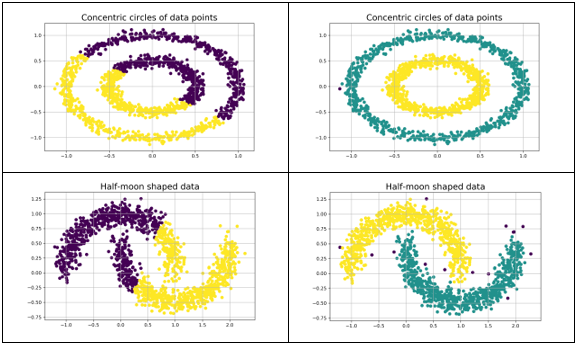
\includegraphics[width=2.5in]{images/kM_DBSCAN.png}
  \caption{Clusters created by k-Means and DBSCAN.
  First Column : k-Means, Second Column : DBSCAN \newline
  Adapted from CE888 lab6 results.
  }
  \label{fig_cluster}
  \end{figure}

As it can be seen in Figure 1, k-Means algorithm can not cluster non-linear data. Results in \cite{xie2016unsupervised} also confirm that, but it also shows us that the k-Means can be significantly improved if the dimensions of the data is reduced before the clustering procedure. In \cite{salakhutdinov2007learning} a multilayer network is used to map high dimensional, non-linear features to low-dimensional space which is fine-tuned to work with KNN. They achieved 1.01\% error rate using 7 nearest neighbours on MNIST dataset.\par

The study \cite{hinton2006reducing} gives a lot of insight on autoencoders and dimensionality reduction. They introduce the pre-training notion, which involves an effective way of initializing good weights and training the network layer by layer. Then they suggest fine-tuning the deep network as a whole. This practice can also be seen in \cite{vincent2010stacked} and \cite{xie2016unsupervised}, these studies also suggest pre-training. On the other hand, \cite{ma2015deep} concludes that the pre-training procedure does not improve the accuracy. Their experiments show that the pre-training, over multiple DNNs and 15 different datasets, on average reduce the accuracy. Another study\cite{poultney2007efficient} learns overcomplete representations of features for data reconstructions. It is shown in their results that this sparse, energy based autoencoder with linear layers can reproduce the MINST dataset with 0.7\% error, while not requiring any preprocessing.\cite{le2011building} also follows a similar approach, in which a deep sparse network trained in unsupervised fashion to recognize faces, humans and objects.
Finally, the last study we looked at implemented and compared different models (Figure 2). As a result \cite{coates2011analysis} states that the best result obtained came from k-Means clustering.

\begin{table}[!ht]
  %% increase table row spacing, adjust to taste
  \renewcommand{\arraystretch}{1.3}
  % if using array.sty, it might be a good idea to tweak the value of
  % \extrarowheight as needed to properly center the text within the cells
  \caption{Test recognition accuracy (and error) for
  NORB dataset.\newline
  Adapted from : \cite{coates2011analysis} }
  \label{tab_coates_res}
  \centering
  %% Some packages, such as MDW tools, offer better commands for making tables
  %% than the plain LaTeX2e tabular which is used here.
  \begin{tabular}{|c||c|}
  \hline
  Algorithm  &     Accuracy (error) \\
  \hline
  \hline
  Conv. Neural Network &    93.4\% (6.6\%)\\
  Deep Boltzmann Machine &      92.8\ (7.2\%)\\
  Deep Belief Network&    95.0\% (5.0\%)\\
  Deep neural network &    97.13\% (2.87\%)\\
  \hline
  Sparse auto-encoder &    96.9\% (3.\%)\\
  Sparse RBM &    96.2\ (3.8\%)\\
  K-means clustering ( 4000 features) &   97.21\% (2.79\%)\\
  \hline
  \end{tabular}
  \end{table}


\section{Methodology}
Our main goal in this study is to correctly cluster data using unsupervised machine learning techniques.
To accomplish this task we will go through three different subtasks. First, we will use traditional clustering algorithms 
to see how they perform on our datasets. In the second part, we will use autoencoders to learn good features
from our datasets, then we will pass the- extracted features- outputs of the autoencoder to a clustering algorithm to see the difference
in their performance. Finally, we will change the output activation function of the autoencoder to the softmax 
activation function, which will give us the probability distribution of the output vector. Then we will use
the maximum weighted class as our cluster assignment.\par
Before starting the experiments the datasets will be examined and processed appropriately for each sub-task.
For the first sub task, depending on the complexity and dimensions of the given data, a suitable clustering algorithm will be chosen.
For the second sub-task, features of the datasets will be standardized. As LeCun concludes in \cite{lecun2012efficient}, networks
can learn better and faster if the inputs are centered around zero with equalized covariance. Another consideration for sub-tasks
two and three is using ensemble of autoencoders. Since the optimization of the randomly initialized weights is 
difficult \cite{hinton2006reducing}, we can have multiple autoencoders in our model to mitigate the effects of random weight initialization.
For the last sub-task, since we will be using softmax as our activation function, the targets of our datasets will be 
converted to one hot coded versions.\par

The three datasets chosen to be clustered in this study are Modified NIST, Human Activity Recognition Using Smartphones (HAR) 
and High Time Resolution Universe Survey 2 (HTRU2).\par

MNIST is a image dataset of hand written digits. It is a modified version of the NIST dataset collected from Census Bureau employees and high-school
students and processed by LeCun et.al..The original NIST set was normalized, so that each sample would be centered
according to the weights of it's pixels in a 28x28 box. Images were also converted to grey-scale and shuffled to make it
easy to use in machine learning applications \cite{lecun1998gradient}. The dataset consists of 60.000 training images and 10.000 test images. Since each
sample is represented as a 28x28 pixel binary image, it can be said that samples have 784 features. MNIST dataset is frequently
used in machine learning research[--], which makes it easier for researchers to compare their models and solutions to the others
in the field.

\begin{figure}[!ht]
\centering
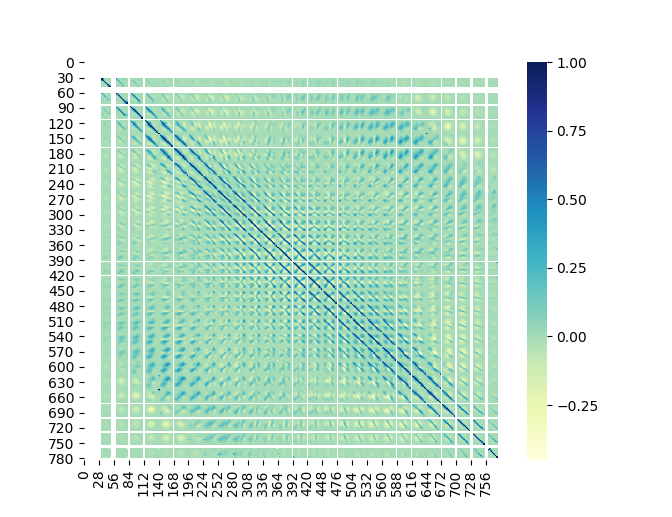
\includegraphics[width=2.5in]{images/cor_heat_mnist.png}
\caption{Corraletion heatmap of MNIST features.}
\label{fig_mnist}
\end{figure}

HAR is a dataset of multiple classes of human activities. It was created by recording different classes of activities of 30 volunteers
by using the accelerometer and the gyroscope in a smartphone. These sensors were used to record the linear acceleration and angular velocity
on three axes at 50 Hz. Volunteers were also recorded by a camera for the labeling of the activities(walking, walking upstairs, walking downstairs, sitting, standing, laying)\cite{anguita2013public}. The dataset consists of 7352
training samples and 2947 test samples. Each sample has 561 features which are- extracted- estimated from the recorded accelerometer and gyroscope signals.These features are normalized, scaled and shifted to be within [-1,1].  Subject id labels for the features and mentioned raw accelerometer and gyroscope signals are also provided with the dataset.
Dimensions of the subject ids are the same with their training and testing parts. On the other hand, the raw signals are seperated into nine different files grouped under three axes, which are body acceleration (X,Y,Z), body gyroscope (X,Y,Z) and total acceleratin (X,Y,Z).

\begin{figure}[!ht]
  \centering
  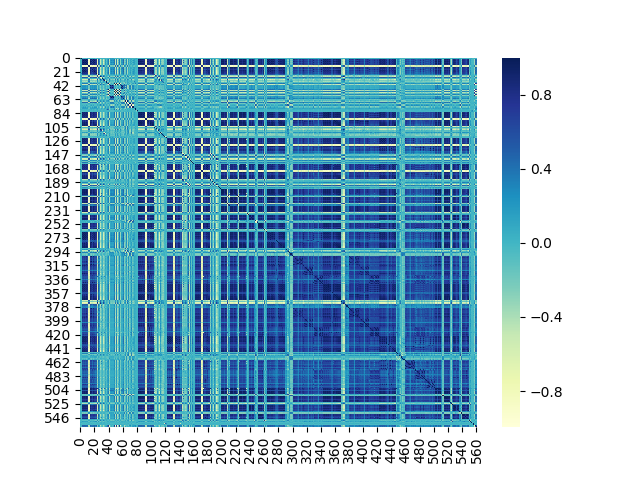
\includegraphics[width=2.5in]{images/cor_heat_har.png}
  \caption{Corraletion heatmap of HAR features.}
  \label{fig_har}
  \end{figure}
  \par
  
  Our last dataset HTRU2 was obtained by Bates\cite{bates2012high} using ANNs to first filter out the bad candidates,then manually inspecting the outputs of the ANN.Each sample of HTRU2 is a set of features extracted from the data acquired by large radio telescopes during High Time Resolution Universe Survey. HTRU2 has 8 features and consists of 17,898 total samples. Only 1,639 of them are positive pulsar samples and the 16,259 of them are negative samples. The first four features are simple statistics of the pulsar profiles and rest of the features were obtained from DM-SNR curve\cite{keith2010high}.These compact features were obtained from 90.000 labeled pulsar candidates by using Pulsar Feature Lab \cite{Lyon2015}.

  \begin{figure}[!ht]
    \centering
    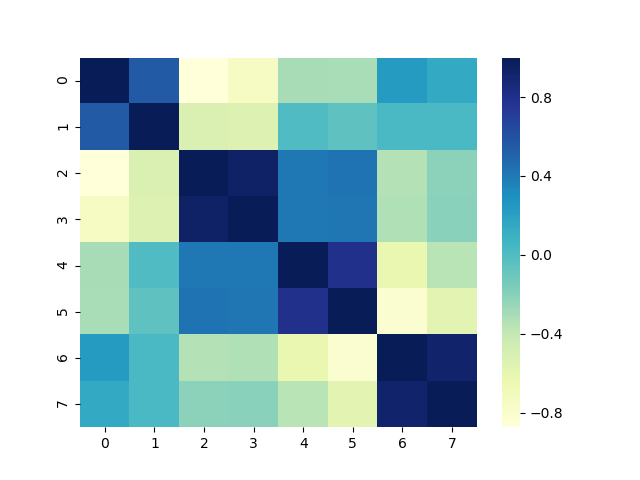
\includegraphics[width=2.5in]{images/cor_heat_htru.png}
    \caption{Corraletion heatmap of htru features.}
    \label{fig_htru}
    \end{figure}
    \par
  
  \begin{table}[!ht]
  %% increase table row spacing, adjust to taste
  \renewcommand{\arraystretch}{1.3}
  % if using array.sty, it might be a good idea to tweak the value of
  % \extrarowheight as needed to properly center the text within the cells
  \caption{Dataset statistics.}
  \label{tab_datasets}
  \centering
  %% Some packages, such as MDW tools, offer better commands for making tables
  %% than the plain LaTeX2e tabular which is used here.
  \begin{tabular}{|c||c|c|c|}
  \hline
  Datasets &    Data Points &  Features &  Classes \\
  \hline
  \hline
  MNIST &    70.000 &   784 &                 10 \\
  \hline
  HAR &       10.299 &   561 &                 6 \\
  \hline
  HTRU2 &    17,898 &   8 &                  2 \\
  \hline
  \end{tabular}
  \end{table}
\section{Experiments}

In the experiments the implementation of the tasks and data analysis will be done using python. In the imlementation of the traditional clustering algorithms, sckit-learn library will be used because of its easy to use nature and rich functions. For the rest of the tasks, tensorflow and keras libraries will be used to implement autoencoders, since tensorflow converts the python code into C code in runtime, it is fast and it can run on GPUs, making it one of the best neural network library. Finally, the data analysis and plotting will be done using matplotlib and seaborn libraries.

\subsection{Clustering Algorithms}
In the core part of the clustering experiments, k-Means and DBSCAN algorithms will be used. These algorithms will be first compared to each other, then their results will be analysed, evaluated and recorded for future comparisons. If there is enough time to deviate from the core path, agglomerative clustering algorithm will also be used and these clustering algorithms will be tested again after applying dimensionality reduction methods like PCA/kernel PCA, LDA to the datasets. Given enough time, we will try these dimension reduction algorithms to confirm\cite{baldi1989neural}, in which it is concluded that the linear autoencoders with squared loss functions behave like PCAs. Otherwise, the experiments will continue with the autoencoders.  

\subsection{AutoEncoder and Softmax}
Rest of the tasks share a similar model. Both of them will be using autoencoders to extract features. Implementation priority will be given to the main parts. First, an autoencoder will be trained and optimized to learn good features, then the output of these features will be passed to the mentioned clustering algorithms in the first task. Then, in the second part the output activations will be swapped with softmax activation function for clustering.\par
After implementing the minimum requirements, if there is enough time, various additional experiments will be performed. First, we will use linear autoencoder with one hidden layer for clustering to compare the performance to clustering with PCA. Then, we will perform the same experiment for non-linear autoencoder and kernel PCA. After the comparisons, we will try methods like Dropout\cite{srivastava2014dropout} and denoising, to prevent one to one mapping and promote generalization\cite{vincent2010stacked}. Finally we will experiment with ensemble of autoencoders for more robust results. 

\subsection{Similar Work}

In the study\cite{hinton2006reducing}, autoencoders are compared to non-linear PCA and other dimensionality reduction methods. And it is stated that the autoencoders out perform PCA, logistic PCA, latent semantic analysis (LSA) and locar linear embedding techniques. The results of the reconstructions of MNIST digits from the study can be seen below.

\begin{figure}[!ht]
  \centering
  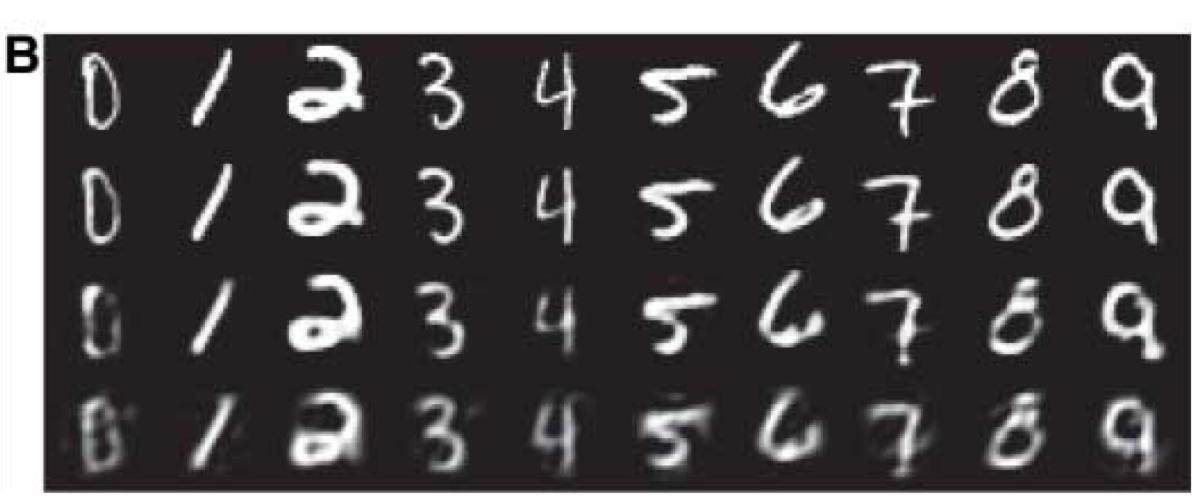
\includegraphics[width=2.5in]{images/hinton_mnist.png}
  \caption{Top to bottom: Random test images, autoencoder reconstruction, logistic PCA reconstruction and standart PCA reconstruction.\newline Adapted from : \cite{hinton2006reducing}}
  \label{fig_hinton_mnist}
  \end{figure}

  \par

Another study \cite{xie2016unsupervised} uses autoencoders with dropout to extract good features for clustering.
In their model, softmax is applied to the resulting output vector from the autoencoder and then they optimize the network by comparing the soft assignment to the target clusters. Their results on MNIST can be seen below. 

\begin{table}[!ht]
  %% increase table row spacing, adjust to taste
  \renewcommand{\arraystretch}{1.3}
  % if using array.sty, it might be a good idea to tweak the value of
  % \extrarowheight as needed to properly center the text within the cells
  \caption{Clustering accuracy on different subsamples of MNIST\newline
  Adapted from: \cite{xie2016unsupervised}}
  \label{tab_res_clus}
  \centering
  %% Some packages, such as MDW tools, offer better commands for making tables
  %% than the plain LaTeX2e tabular which is used here.
  \begin{tabular}{|c||c|c|c|c|c|c|}
  \hline
   Method  &    0.1 &  0.3 &  0.5 & 0.7 &  0.9  \\
  \hline
  \hline
  k-Means &    47.14\% &   49.93\% &     53.65\%   &    54.16\%  &   54.39\% \\
  \hline
  AE + k-Means & 66.82\% &   74.91\% &     77.93\%   &    80.04\%  &   81.31\% \\
  \hline
  DEC(proposed) &  70.10\% &   80.92\% &     82.68\%   &    84.69\%  &   85.41\% \\
  \hline
  \end{tabular}
  \end{table}

% Note that the IEEE typically puts floats only at the top, even when this
% results in a large percentage of a column being occupied by floats.


% An example of a double column floating figure using two subfigures.
% (The subfig.sty package must be loaded for this to work.)
% The subfigure \label commands are set within each subfloat command,
% and the \label for the overall figure must come after \caption.
% \hfil is used as a separator to get equal spacing.
% Watch out that the combined width of all the subfigures on a 
% line do not exceed the text width or a line break will occur.


% Note that often IEEE papers with subfigures do not employ subfigure
% captions (using the optional argument to \subfloat[]), but instead will
% reference/describe all of them (a), (b), etc., within the main caption.
% Be aware that for subfig.sty to generate the (a), (b), etc., subfigure
% labels, the optional argument to \subfloat must be present. If a
% subcaption is not desired, just leave its contents blank,
% e.g., \subfloat[].


% An example of a floating table. Note that, for IEEE style tables, the
% \caption command should come BEFORE the table and, given that table
% captions serve much like titles, are usually capitalized except for words
% such as a, an, and, as, at, but, by, for, in, nor, of, on, or, the, to
% and up, which are usually not capitalized unless they are the first or
% last word of the caption. Table text will default to \footnotesize as
% the IEEE normally uses this smaller font for tables.
% The \label must come after \caption as always.
%
% \begin{table}[!t]
% %% increase table row spacing, adjust to taste
% \renewcommand{\arraystretch}{1.3}
% % if using array.sty, it might be a good idea to tweak the value of
% % \extrarowheight as needed to properly center the text within the cells
% \caption{An Example of a Table}
% \label{table_example}
% \centering
% %% Some packages, such as MDW tools, offer better commands for making tables
% %% than the plain LaTeX2e tabular which is used here.
% \begin{tabular}{|c||c|}
% \hline
% One & Two\\
% \hline
% Three & Four\\
% \hline
% \end{tabular}
% \end{table}




\section{Discussion}

At the end of the experiments, the evaluation of each model's cluster assignments will be calculated by using the V-measure. Since it takes into account both completeness and homogenity of the clusters, it will be our choice of evaluation\cite{rosenberg2007v}. On the other hand we will also use the Fowlkes-Mallows score. Because it allows us to compare the performance of our three different methods\cite{fowlkes1983method}. Also as an addition, we plan to evaluate the contingency matrix of each model, then perform McNemar's test between the models to see the significance of their difference.\par

This study will improve our understanding of autoencoders and it will give us a chance to observe how they perform compared to the traditional methods. It is assumed that the task of optimizing and fine tuning the encoders will be difficult and time consuming. Another benefit will be the comparison of the softmax clustering to the rest of the methods. Downside of this study will be understanding why the autoencoder does what it does, since it is a black box model. Luckily this is out of the scope of this study. 

In a broader perspective, these experiments will improve our understanding of clustering, data manipulation and unsupervised learning in general. Understanding the data, its complexity and dimensions are not trivial yet very important. Even though Machine Learning and Data Science fields can provide many models and tools, it is difficult to get good results if we are not familiar with the data/problem we are dealing with.\par

\section{Conclusion}

We briefly explained the purpose and the tasks of the project. While going through the literature, importance of unsupervised learning was understood. Also it was realized that the field needs more attention. Later on, we described our model and the datasets we are going to use. Then the experiments we are going to perform were described with references to the similar work.In the end the evaluation methods that we will use were explained together with what we expect to gain at the end of this work.\par

We believe that this work will provide a lot of insights and practical experiences about clustering, autoencoders and data analysis. With the addition of improving our data presentation skills, such as drawing graphs and plots through software. This will be a good study to put what we learned in theory to practice, do the experiments for ourselves and compare our results to the ones we found. 
\newpage



% if have a single appendix:
%\appendix[Proof of the Zonklar Equations]
% or
%\appendix  % for no appendix heading
% do not use \section anymore after \appendix, only \section*
% is possibly needed

% use appendices with more than one appendix
% then use \section to start each appendix
% you must declare a \section before using any
% \subsection or using \label (\appendices by itself
% starts a section numbered zero.)
%


\appendices

\section{}

See page 6 for the GANTT chart of the assignment. 

% you can choose not to have a title for an appendix
% if you want by leaving the argument blank

\newpage

% trigger a \newpage just before the given reference
% number - used to balance the columns on the last page
% adjust value as needed - may need to be readjusted if
% the document is modified later
%\IEEEtriggeratref{8}
% The "triggered" command can be changed if desired:
%\IEEEtriggercmd{\enlargethispage{-5in}}

% references section

% can use a bibliography generated by BibTeX as a .bbl file
% BibTeX documentation can be easily obtained at:
% http://mirror.ctan.org/biblio/bibtex/contrib/doc/
% The IEEEtran BibTeX style support page is at:
% http://www.michaelshell.org/tex/ieeetran/bibtex/
\bibliographystyle{IEEEtran}

\bibliography{refs}
%
\newpage

\begin{landscape}
  \begin{figure}[!h]
     \centering
      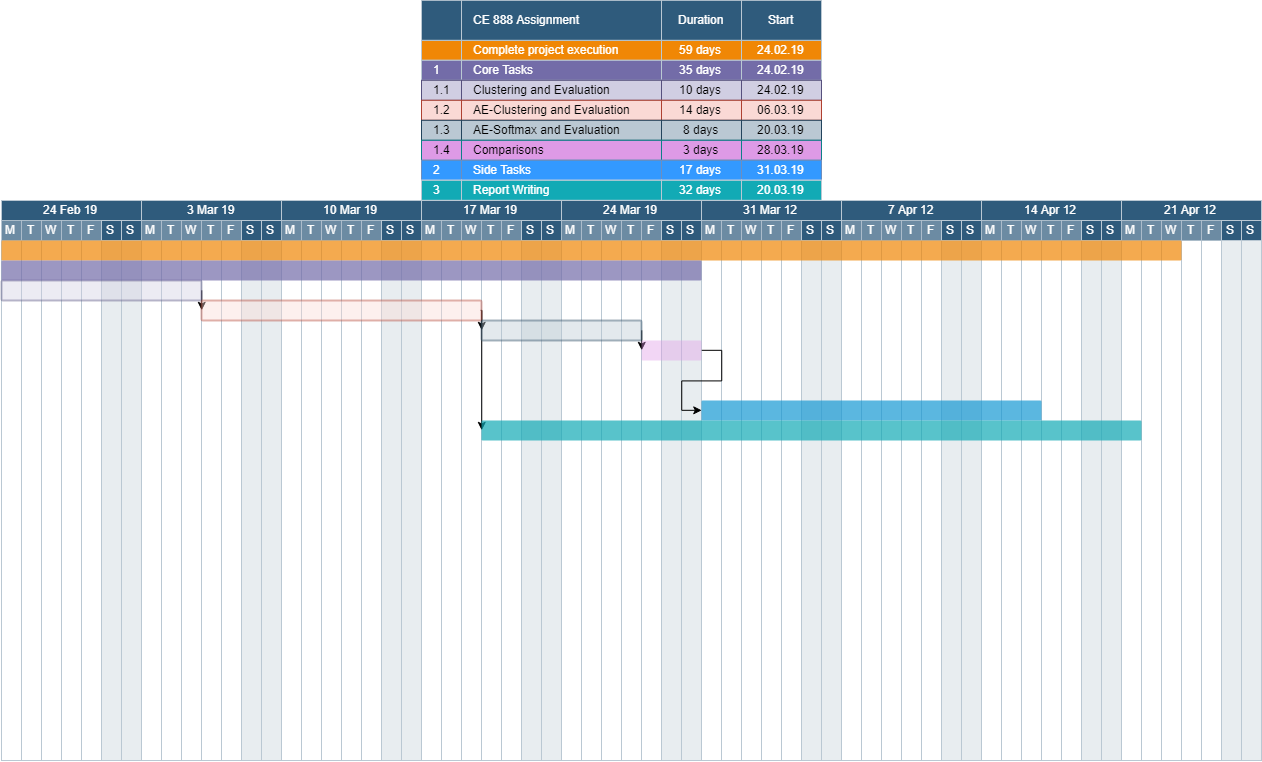
\includegraphics[width=1.25\textwidth,height=0.90\textheight]{g_chart.png}
      \caption{Assignment GANTT Chart}
      \label{fig_g_chart}
  \end{figure}
  \end{landscape}
% biography section
% 
% If you have an EPS/PDF photo (graphicx package needed) extra braces are
% needed around the contents of the optional argument to biography to prevent
% the LaTeX parser from getting confused when it sees the complicated
% \includegraphics command within an optional argument. (You could create
% your own custom macro containing the \includegraphics command to make things
% simpler here.)
%\begin{IEEEbiography}[{\includegraphics[width=1in,height=1.25in,clip,keepaspectratio]{mshell}}]{Michael Shell}
% or if you just want to reserve a space for a photo:




% that's all folks
\end{document}